%iffalse
\let\negmedspace\undefined
\let\negthickspace\undefined
\documentclass[journal,12pt,onecolumn]{IEEEtran}
\usepackage{cite}
\usepackage{amsmath,amssymb,amsfonts,amsthm}
\usepackage{algorithmic}
\usepackage{graphicx}
\usepackage{textcomp}
\usepackage{xcolor}
\usepackage{txfonts}
\usepackage{listings}
\usepackage{enumitem}
\usepackage{mathtools}
\usepackage{gensymb}
\usepackage{comment}
\usepackage[breaklinks=true]{hyperref}
\usepackage{tkz-euclide} 
\usepackage{listings}
\usepackage{gvv}                                        
%\def\inputGnumericTable{}                                 
\usepackage[latin1]{inputenc}                                
\usepackage{color}                                            
\usepackage{array}                                            
\usepackage{longtable}                                       
\usepackage{calc}                                             
\usepackage{multirow}                                         
\usepackage{hhline}                                           
\usepackage{ifthen}                                           
\usepackage{lscape}
\usepackage{tabularx}
\usepackage{array}
\usepackage{float}


\newtheorem{theorem}{Theorem}[section]
\newtheorem{problem}{Problem}
\newtheorem{proposition}{Proposition}[section]
\newtheorem{lemma}{Lemma}[section]
\newtheorem{corollary}[theorem]{Corollary}
\newtheorem{example}{Example}[section]
\newtheorem{definition}[problem]{Definition}
\newcommand{\BEQA}{\begin{eqnarray}}
\newcommand{\EEQA}{\end{eqnarray}}
\newcommand{\define}{\stackrel{\triangle}{=}}
\theoremstyle{remark}
\newtheorem{rem}{Remark}

% Marks the beginning of the document
\begin{document}
\bibliographystyle{IEEEtran}
\vspace{3cm}

\title{2008-EE-18-34}
\author{AI24BTECH11011 - Himani Gourishetty}
\maketitle
\bigskip

\renewcommand{\thefigure}{\theenumi}
\renewcommand{\thetable}{\theenumi}
\begin{enumerate}
    \item A 3-phase Voltage source Inverter is operated in $180{\degree}$  conduction mode.Which one of the following statements is true?
    \begin{enumerate}
        \item Both pole-voltage and line-voltage will have $3^{rd}$ harmonic components
        \item Pole-voltage will have $3^{rd}$ harmonic components but line-voltage will be free from $3^{rd}$ harmonic
         \item Line-voltage will have $3^{rd}$ harmonic components but pole-voltage will be free from $3^{rd}$ harmonic
         \item  Both pole-voltage and line-voltage will be free from $3^{rd}$ harmonic components
    \end{enumerate}
    \item The impulse response of a causal linear time-invariant system is given as $h(t)$. Now consider the following two statements:\\
     Statement (I): Principle of superposition holds\\
     Statement (II): $h(t) = 0$ for $t < 0$\\
     Which one of the following statements is correct?
     \begin{enumerate}
    \item[(A)] Statement (I) is correct and Statement (II) is wrong
    \item[(B)] Statement (II) is correct and Statement (I) is wrong
    \item[(C)] Both Statement (I) and Statement (II) are wrong
    \item[(D)] Both Statement (I) and Statement (II) are correct
    \end{enumerate}
    \item It is desired to measure parameters of 230v/115v,2kVA, single-phase transformer. The following wattmeters are available in a laboratory.\\
    $W_1:$ 250V, 10A, Low Power Factor\\
    $W_2:$ 250v,5A,Low Power Factor\\
    $W_3:$ 150V, 10A, High Power Factor\\
    $W_4:$ 150V, 5A, High Power Factor\\
    The wattmeters used in open circuit test and short circuit test of the transformer will respectively be 
    \begin{enumerate}
        \item $W_1$ and $W_2$
        \item $W_2$ and $W_4$
        \item $W_1$ and $W_4$
        \item $W_2$ and $W_3$
    \end{enumerate}
   \item The time constant of the given circuit will be\\
   \begin{figure}[h!]
   \centering
   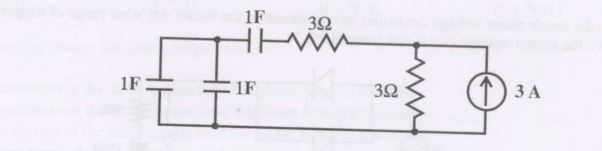
\includegraphics[width=0.7\linewidth]{figs/fig1.jpg}
   \label{fig:11011}
   \end{figure}
   \begin{enumerate}
       \item $\frac{1}{9}$s
       \item $\frac{1}{4}$s
       \item 4s
       \item 9s
       \end{enumerate}
       \item  The resonant frequency of the given circuit will be\\
       \begin{figure}[h!]
       \centering
       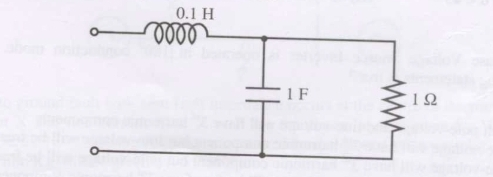
\includegraphics[width=0.7\linewidth]{figs/fig2.jpg}
       \label{fig:11011}
       \end{figure}
       \begin{enumerate}
           \item 1 $\frac{rad}{s}$
           \item 2 $\frac{rad}{s}$
	   \item 3 $\frac{rad}{s}$
           \item 4 $\frac{rad}{s}$
       \end{enumerate}
       \item Assumimg ideal elements in a circuit shown below, the voltage $V_{ab}$ will be\\
       \begin{figure}[h!]
       \centering
       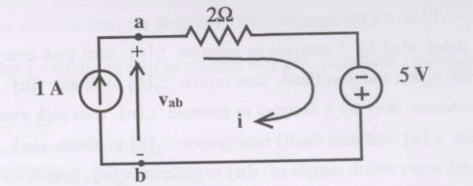
\includegraphics[width=0.7\linewidth]{figs/fig3.jpg}
       \label{fig:11011}
       \end{figure}
       \begin{enumerate}
           \item -3V
           \item 0V
           \item 3V
           \item 5V
       \end{enumerate}
       \item A capacitor consists of 2 metal plates each $500 \times 500 mm^2$ and spaced 6 mm apart. The space between the metal plates is filled with glass plate of 4mm thickness and a layer of paper of 2mm thickness. The relative permittivities of the glass and paper are 8 and 2 respectively. Neglecting the fringing effect, the capacitance will be (Given that $\epsilon_{0}=8.85\times 10^{-12}\frac{F}{m}$)
       \begin{enumerate}
           \item 983.33pF
           \item 1475 pF
           \item 6637.5 pF
           \item 9956.25 pF
       \end{enumerate}
      \item A coil of 300 turns is wound on a non -magnetic core having a mean circumference of 300mm and a cross-sectional area of $300 mm^2$. The inductance of the coil corresponding to a magnetizing current of 3A will be (Given that $\mu_0=4\pi\times10^{-7}$)
      \begin{enumerate}
      \item $37.68\mu H$
      \item $113.04\mu H$
      \item 37.68 mH
      \item 113.04 mH
      \end{enumerate}
      \item In the circuit shown in the figure, the value of the current i will be given by
      \begin{figure}[h!]
      \centering
      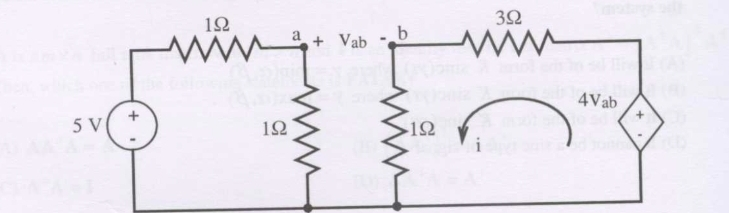
\includegraphics[width=0.7\linewidth]{figs/fig4.jpg}
      \label{fig:11011}
      \end{figure}
      \begin{enumerate}
          \item 0.31A
          \item 1.25A
          \item 1.75A
          \item 2.5A
      \end{enumerate}
      \item Two point charges $Q_1=10\mu C$ and $Q_2=20 \mu C$ are placed at coordinates $\brak{1,1,0}$ and $\brak{-1,-1,0}$ respectively. The total electric flux passing through a plane $z=20$ will be
      \begin{enumerate}
          \item $7.5\mu C$
          \item $135 \mu C$
          \item $15.0 \mu C$
          \item $22.5 \mu C$
      \end{enumerate}
      \item Given a sequence $x[n]$, to generate the sequence $y[n]=x[3-4n]$, which one of the folllowing procedures would be correct?
      \begin{enumerate}
          \item First delay x[n] by 3 samples to generate $z_1[n]$, then pick every $4^{th}$ sample of $z_1[n]$ to generate $z_2[n]$, and then finally time reverse $z_2[n]$ to obtain y[n]
          \item First advance x[n] by 3 samples to generate $z_1[n]$, then pick every $4^{th}$ sample of $z_1[n]$ to generate $z_2[n]$, and then finally time reverse $z_2[n]$ to obtain y[n]
          \item First pick every fourth sample of x[n] to generate $V_1[n]$, time-reverse $v_1[n]$ to obtain $v_2[n]$, and finally advance $v_2[n]$ by 3 samples to obtain y[n]
          \item  First pick every fourth sample of x[n] to generate $V_1[n]$, time-reverse $v_1[n]$ to obtain $v_2[n]$, and finally delay $v_2[n]$ by 3 samples to obtain y[n]
      \end{enumerate}
      \item A system with input $x\brak{t}$ and output $y\brak{t}$ is defined by the input-output relation:
      \begin{align}
          y\brak{t}=\int_{-\infty}^{-2t}x\brak{\tau}d\tau
      \end{align}
      The system will be 
      \begin{enumerate}
          \item casual,time-invariant and unstable
          \item casual, time-invariant and stable
          \item non-casual,time-invariant and unstable
          \item non-casual, time-invariant and unstable
      \end{enumerate}
      \item A signal $x\brak{t}=\sin c\brak{\alpha t}$ where $\alpha$ is a real constant $\brak{\sin c\brak{x}=\frac{\sin\brak{\pi x}}{\pi x}}$ is the input to a Linear Time invariant system whose impulse response $h\brak{t}=\sin c\brak{\beta t}$ where $\beta$ is a real constant. If $min\brak{\alpha,\beta}$ denotes the minimum of $\alpha$ and $\beta$, and similarly $max\brak{\alpha,\beta}$ denotes the maximum of $\alpha$ and $\beta$, and K is a constant, which one of the following statements is true about the \textbf{output of the system}?
      \begin{enumerate}
          \item It will be of the form $K\sin c\brak{\gamma t}$ where $\gamma=min\brak{\alpha,\beta}$
           \item It will be of the form $K\sin c\brak{\gamma t}$ where $\gamma=max\brak{\alpha,\beta}$
           \item It will be of the form $K \sin c\brak{\alpha t}$
           \item It cannot be a $\sin c$ type of signal
      \end{enumerate}
      \item Let $x\brak{t}$ be  a periodic signal with time period T. let $y\brak{t}=x\brak{t-t_0}+x\brak{t+t_0}$ for some $t_0$. The Fourier Series coefficients of $y\brak{t}$ are denoted by $b_k$. If $b_k=0$ for all odd k, then $t_0$ can be equal to 
      \begin{enumerate}
          \item $\frac{T}{8}$
          \item $\frac{T}{4}$
          \item $\frac{T}{2}$
          \item $2T$
      \end{enumerate}
      \item $H\brak{z}$ is a transfer function of a real system. When a signal $x[n]=\brak{1+j}^n$ is the input to such a system, the output is zero. Further, the Region of Convergence (ROC) of $\brak{1-\frac{1}{2}z^{-1}}H\brak{z}$ is the entire Z-plane (except $z=0$). It can then be inferred that $H\brak{z}$ can have a minimum of
      \begin{enumerate}
          \item one pole and one zero
          \item one pole and two zeros
          \item two poles and one zero
          \item two poles and two zeros
      \end{enumerate}
      \item Given $X\brak{z}=\frac{z}{\brak{z-a}^2}$ with $\abs{z}>a$, the residue of $X\brak{z}z^{n-1}$ at $z=a$ for $n\geq 0$ will be
      \begin{enumerate}
          \item $a^{n-1}$
          \item $a^n$
          \item $n a^n$
          \item $na^{n-1}$
      \end{enumerate}
      \item Consider function $f\brak{x}=\brak{x^2-4}^2$ where $x$  is a real number. Then the function has
      \begin{enumerate}
          \item only one minimum
          \item only two minima
          \item three minima
          \item three maxima
      \end{enumerate}
\end{enumerate}
\end{document}

